
\section*{Mesh \& Hacking}
\DefineNamedColor{named}{eclipsered}{rgb}{0.186,0.166,0.182}
\definecolor{tablecolor}{named}{eclipsered}


\begin{eptable}{ l | X }
   \epheader{2}{General Usage}
   % Addiction & Needs fix or receive negative modifier.\\
   AR Mist & In ad-spammed area, up to \modifier{-30} general modifier.\\
   AR Filter & Counter AR mist with \skill{Interface} test.\\
   Hidden Tags & At least \skill{Interface} test at \modifier{-30} to find, maybe impossible.\\
   List Public Devices & Trivial activity.\\
   List Stealthed Devices & Opposed \skill{Interface} test at \modifier{-30} for searcher.\\
   Overloaded Devices & Up to \modifier{-30} if app exceeds device, or device impaired.\\
   Sniffing & Needs \textit{Sniffer} app, \skill{Hacking} test.\\
   Sniffing VPNs & Applies \modifier{-30}, only valid for \dice{1d6} minutes.\\
   Sniffing, Detecting & Defender may make \skill{Infosec} test to detect every minute. \\
\end{eptable}

\bigskip

\subsection*{Accounts and Access}


\begin{eptable}{ l | X }
   \epheader{2}{Accounts}
   % Addiction & Needs fix or receive negative modifier.\\
   Public Account & Does not require login, everyone has access.\\
   User Account & Requires authentication.\\
   Security Account & Can edit logs, modify other user data.\\
   Admin Account & Change all device features, services, shutdown.\\
\end{eptable}

\bigskip

\begin{eptable}{ l | X }
   \epheader{2}{Authentication Methods}
   % Addiction & Needs fix or receive negative modifier.\\
   Biometric Scan & Fingerprint, DNA, retina scan, \ldots\\
   Ego Scan & Brainwave scan with special device.\\
   Direct Neural Interface & Requires special brain implant.\\
   Mesh ID & Just needs the right mesh ID.\\
   Other Account & Account A might grant access to account B.\\
   Passcode & Some secret string, aka \textit{password}.\\
   Passkey & Special physical security token.\\
   Quantum Key & Require passcode delivered on highly secure channel.\\
\end{eptable}

\bigskip

\begin{eptable}{ l | X }
   \epheader{2}{Circumventing Authentication}
   % Addiction & Needs fix or receive negative modifier.\\
   Acquiring Credentials & Get access to actual credential.\\
   Forging Authentication & Might require multiple tests and lengthy times.\\
   Spoofing & Take over connection, see below.\\
\end{eptable}

\begin{itemize}
   \itembox To spoof, first monitor active connection with sniffer.
   \itembox Then take over victim's client with \skill{Hacking} test, complex action. This \textit{only} allows sending. Victim VPN gives \modifier{-30}, Firewall can detect. To also take over victim's server for full-duplex, similar \skill{Hacking} test must succeed.
\end{itemize}

\bigskip


\begin{eptable}{ l | X }
   \epheader{2}{Crypto}
   % Addiction & Needs fix or receive negative modifier.\\
   Public Key & Can be broken with quantum computer, \skill{Infosec} (1 week) task.\\
   Quantum & Cannot be broken, always requires key.\\
\end{eptable}

\bigskip


\begin{eptable}{ l | X }
   \epheader{2}{Universal Actions}
   Access System & Authenticate and access account.\\
   Apply Tag & Mark physical place or thing with AR tag.\\
   Communicate & Mail, text, chat if you have their mesh ID.\\
   Encrypt / Decrypt & Protect or access file if you have key.\\
   Filter AR Mist & Remove AR spam.\\
   Identify Attacker & Detect who is attacking you in mesh combat.\\
   Issue Command & Command a slaved device, ALI or bot with quick action.\\
   Log Off & Exit a system.\\
   Modify Files & Access, modify, delete files (might be recoverable).\\
   Operate Device & Control attached devices, might requires skill test.\\
   Run Script & Run pre-programmed script.\\
   Scan Wireless Signals & Try locate hidden or public devices and their mesh IDs.\\
   Search & Search connected system.\\
   Shield Software & Protect software targeted in mesh combat.\\
   Stealth WiFi Signals & Attempt to hide wireless activity.\\
   Switch Home Device & If infomorph, transfer mind to other system.\\
   Terminate Software & Kill software for which you have access.\\
   Toggle AR Skin & Change looks of world around you.\\
   Toggle Privacy Mode & Set your profile public or private.\\
   Toggle Simulspace & Enter or exit simulspace.\\
   Use Apps & Use installed app, may also require \skill{Interface} test.\\
   Use Service & Access cloud service for which you have access.\\
   View Apps & List all apps you have access to.\\
   View Profile & See profile and rep of anyone not in private mode.\\
   View Sensor Feeds & Access sensor, might also require \skill{Perception} or \skill{Know}.\\
   View System Status & View general system health and activity.\\
\end{eptable}

\bigskip


\begin{eptable}{ l | X }
   \epheader{2}{Security Actions}
   Acquire Mesh ID & View mesh ID of anyone accessing system.\\
   Activate Countermeasure & Trigger countermeasure against spotted attacker .\\
   Attack & Engage against other apps or users.\\
   Bypass Jamming & \skill{Interface} to get short (\SI{3}{s}) transmission through.\\
   Locate Intruder & Identify attacker to system.\\
   Lockout & Block ID (defeat in combat first if signed on).\\
   Monitor Activity & Watch user activity (might require \skill{Infosec}).\\
   Scan Infomorph & Reveal info about infomorph (\skill{Interface}).\\
   Trace & Trace user to physical location.\\
   Trigger Alert & Put system into passive or active alert.\\
   View Logs & View previous user activity.\\
   View Users & View all non-hidden users.\\
\end{eptable}

\bigskip

\begin{eptable}{ l | X }
   \epheader{2}{Admin Actions}
    Disable Systems & Turn off sensors or functions.\\
    Modify Accounts & Add, remove, modify accounts.\\
    Modify Privileges & Modify existing account permissions.\\
    Modify Software & Install, modify or remove software.\\
    Wipe System & Takes 1 to 10 minutes (double for secure wipe).\\
\end{eptable}


% \bigskip

% \begin{eptable}{ X }
%    \epheader{1}{What Your Muse Can}
%     Protect PAN as system defender, shield in mesh combat, launch countermeasures. \\
%     Make research tests to find information. \\
%     Falsify or fluctuate mesh ID. \\
%     Scan newsfeeds for keywords and alerts. \\
%     Teleoperate robots and ALIs. \\
%     xxx. \\
%     xxx. \\
%     xxx. \\
%     xxx. \\
%     xxx. \\
% \end{eptable}

\subsection*{Searches}

\begin{itemize}
   \itembox Looking up common information on mesh is instant and does not require roll.
   \itembox Searches for non-common information on local mesh have timeframe of \SI{1}{h}, and might be complemented by appropriate \skill{Know} skill. Searches outside of the local mesh increase time frame due to distance lag.
   \itembox Superior successes provide more nuanced information, critical success leads to breakthrough understanding, critical failure to false or misleading information.
   \itembox \skill{Research} only yields information. Understanding data might require \skill{Know} test or similar.
   \itembox Searching non-public information (located on specific host or sub-net) requires appropriate access and has special time frame (see table). Encrypted files must be decrypted before they can be searched.
\end{itemize}


\begin{figure}[htbp!]%
   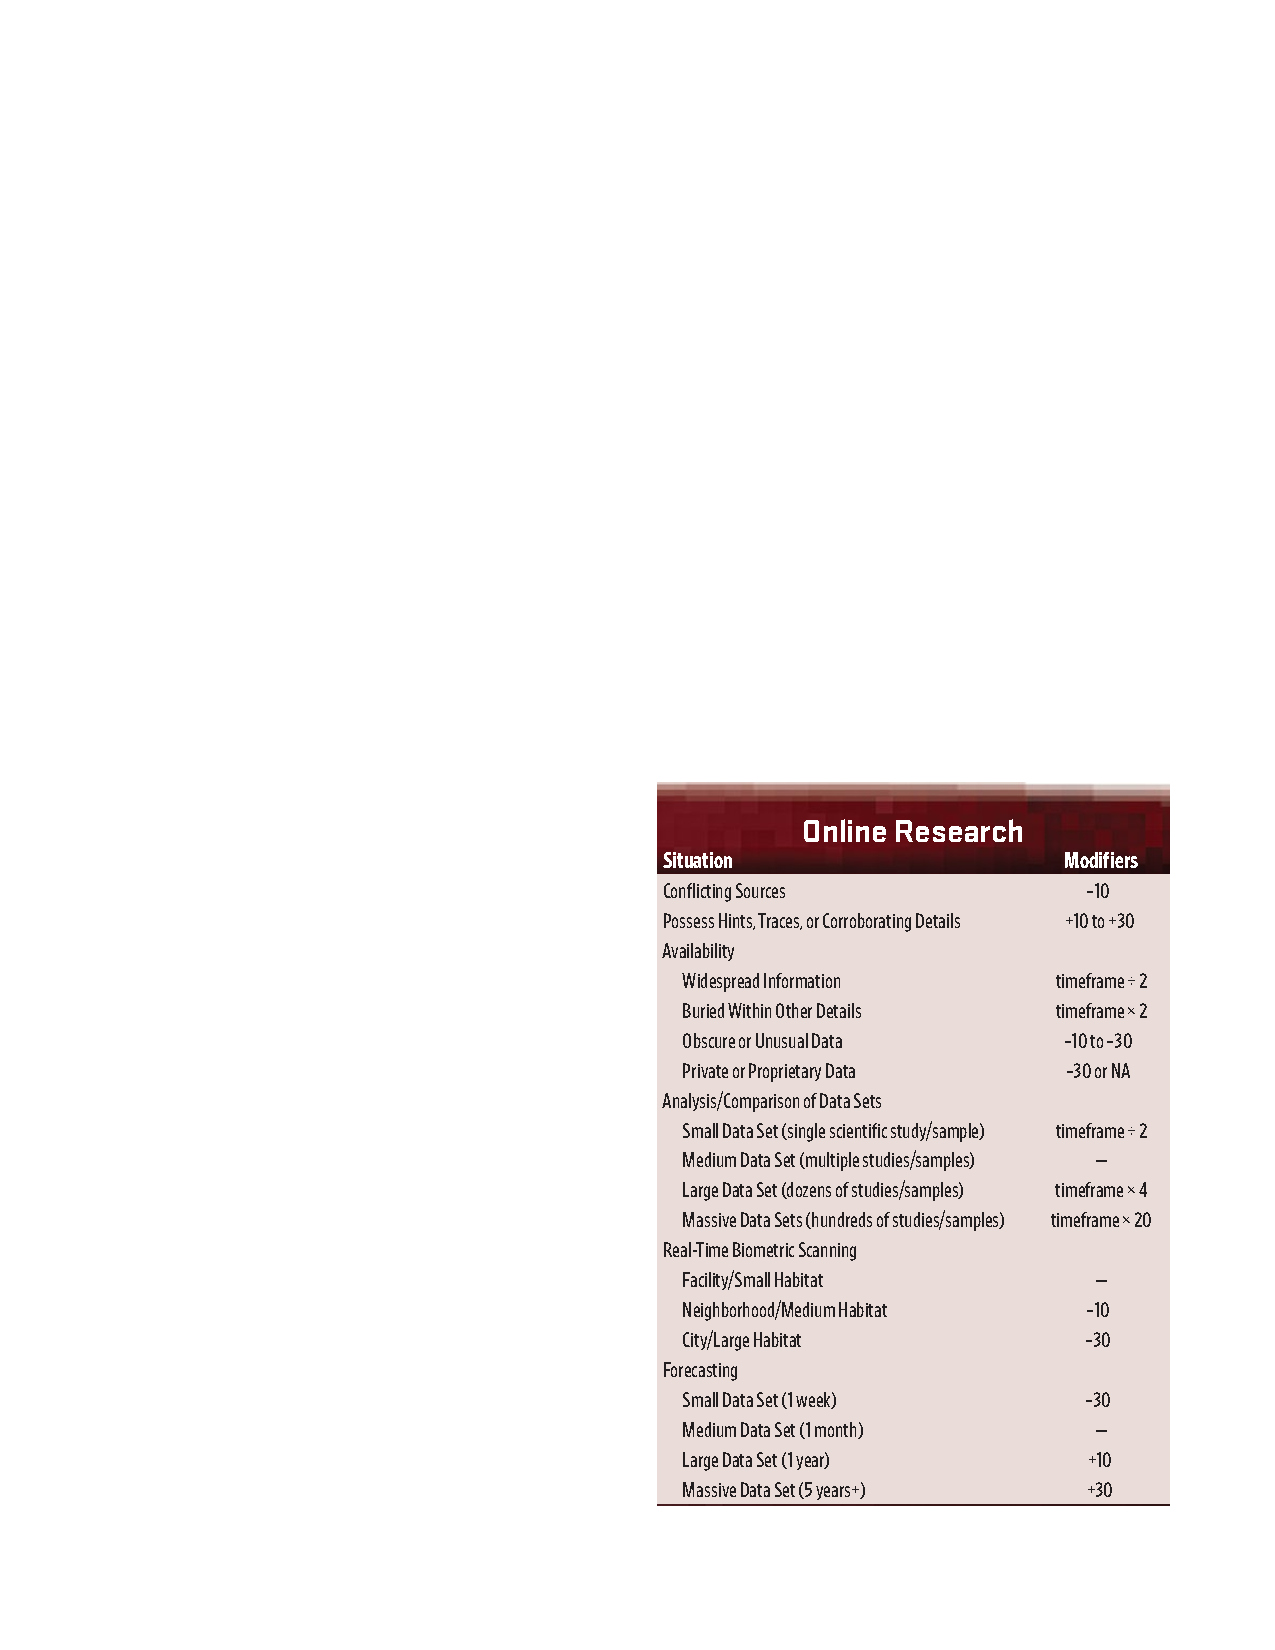
\includegraphics[scale=0.9]{gfx/mesh-research}%
\end{figure}%

\begin{figure}[htbp!]%
   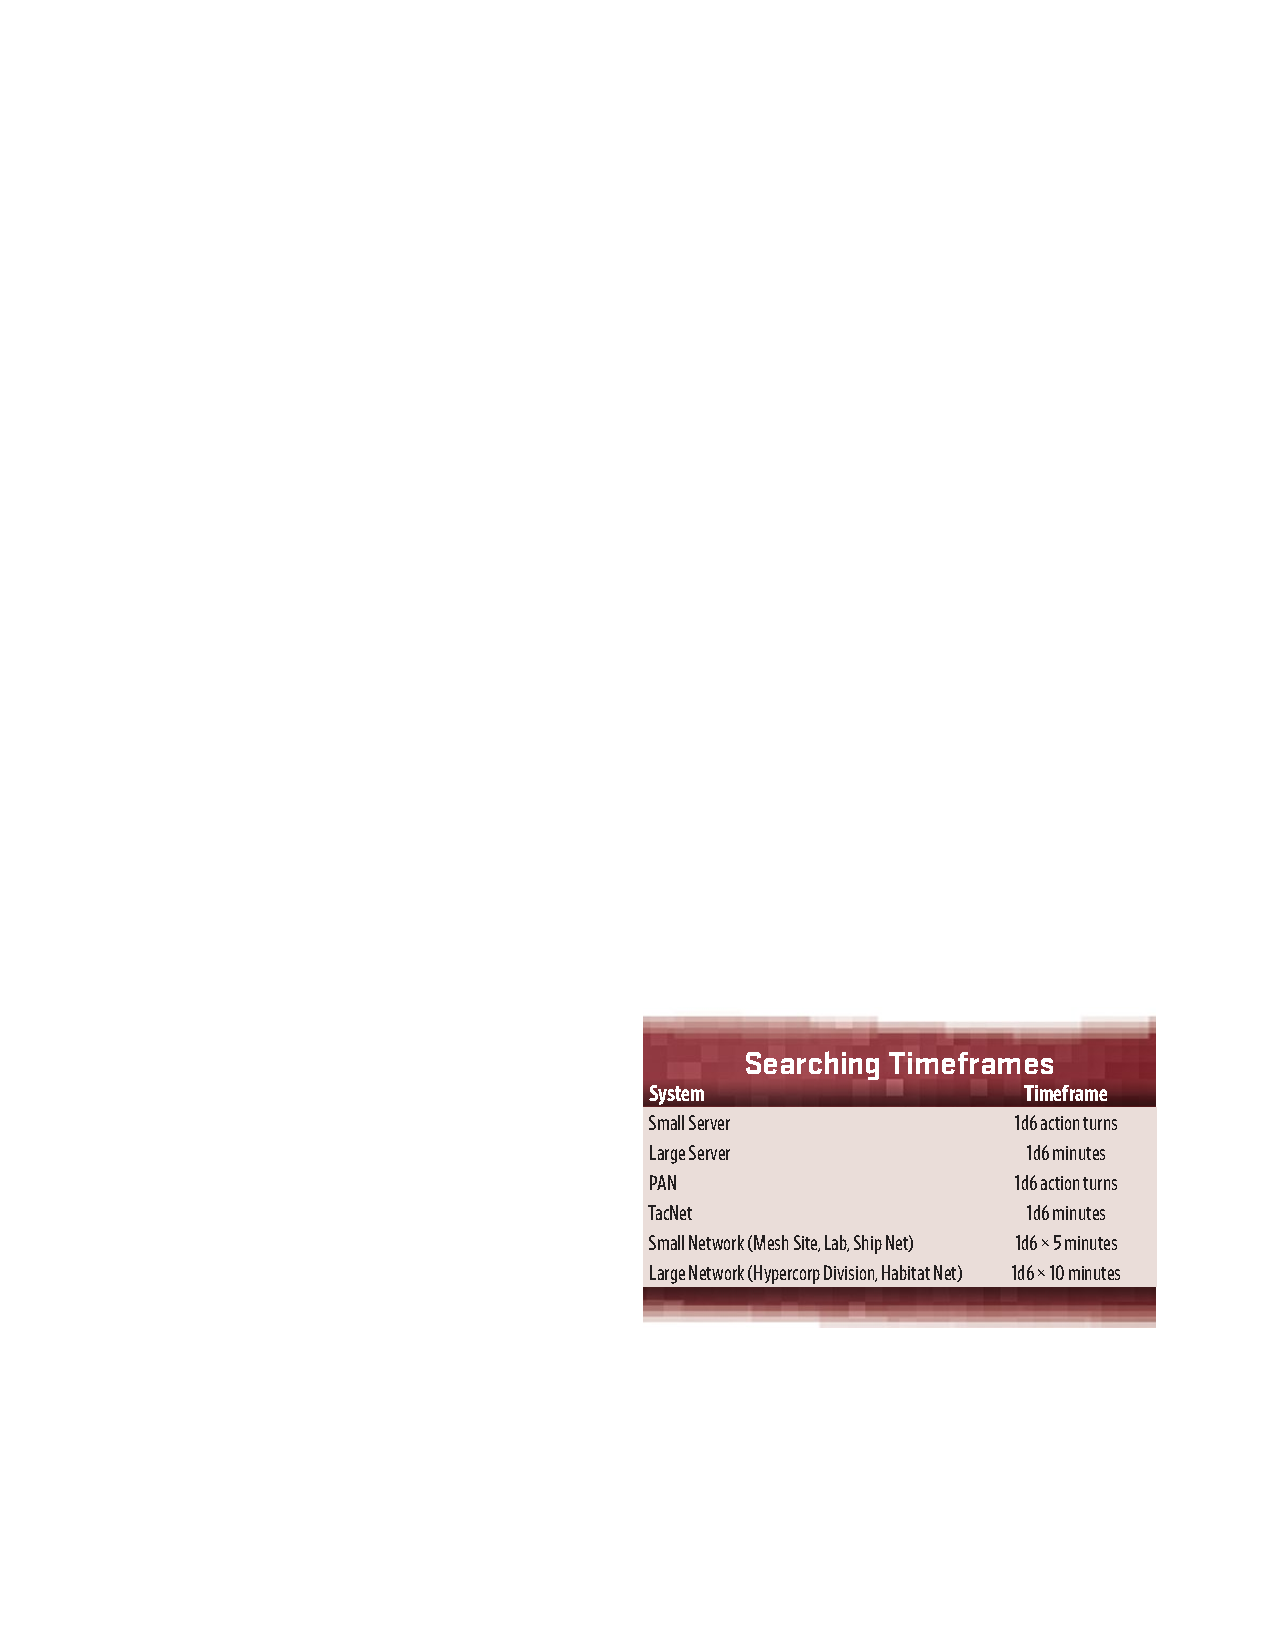
\includegraphics[scale=0.9]{gfx/mesh-search-time}%
\end{figure}%


\subsection*{Physical Tracking}

\begin{itemize}
   \itembox Physical tracking by mesh ID is \skill{Research} and can yield location of target and is instant. If they are in private mode \modifier{-30} modifer, opposed vs \skill{Infosec} if they cycle mesh IDs, timeframe \SI{1}{h}.
   \itembox Biometrical tracking is handled as \skill{Perceive} or \skill{Research}, possibly opposed by \skill{Infiltrate} or \skill{Disguise}.
\end{itemize}


\begin{figure}[htbp!]%
   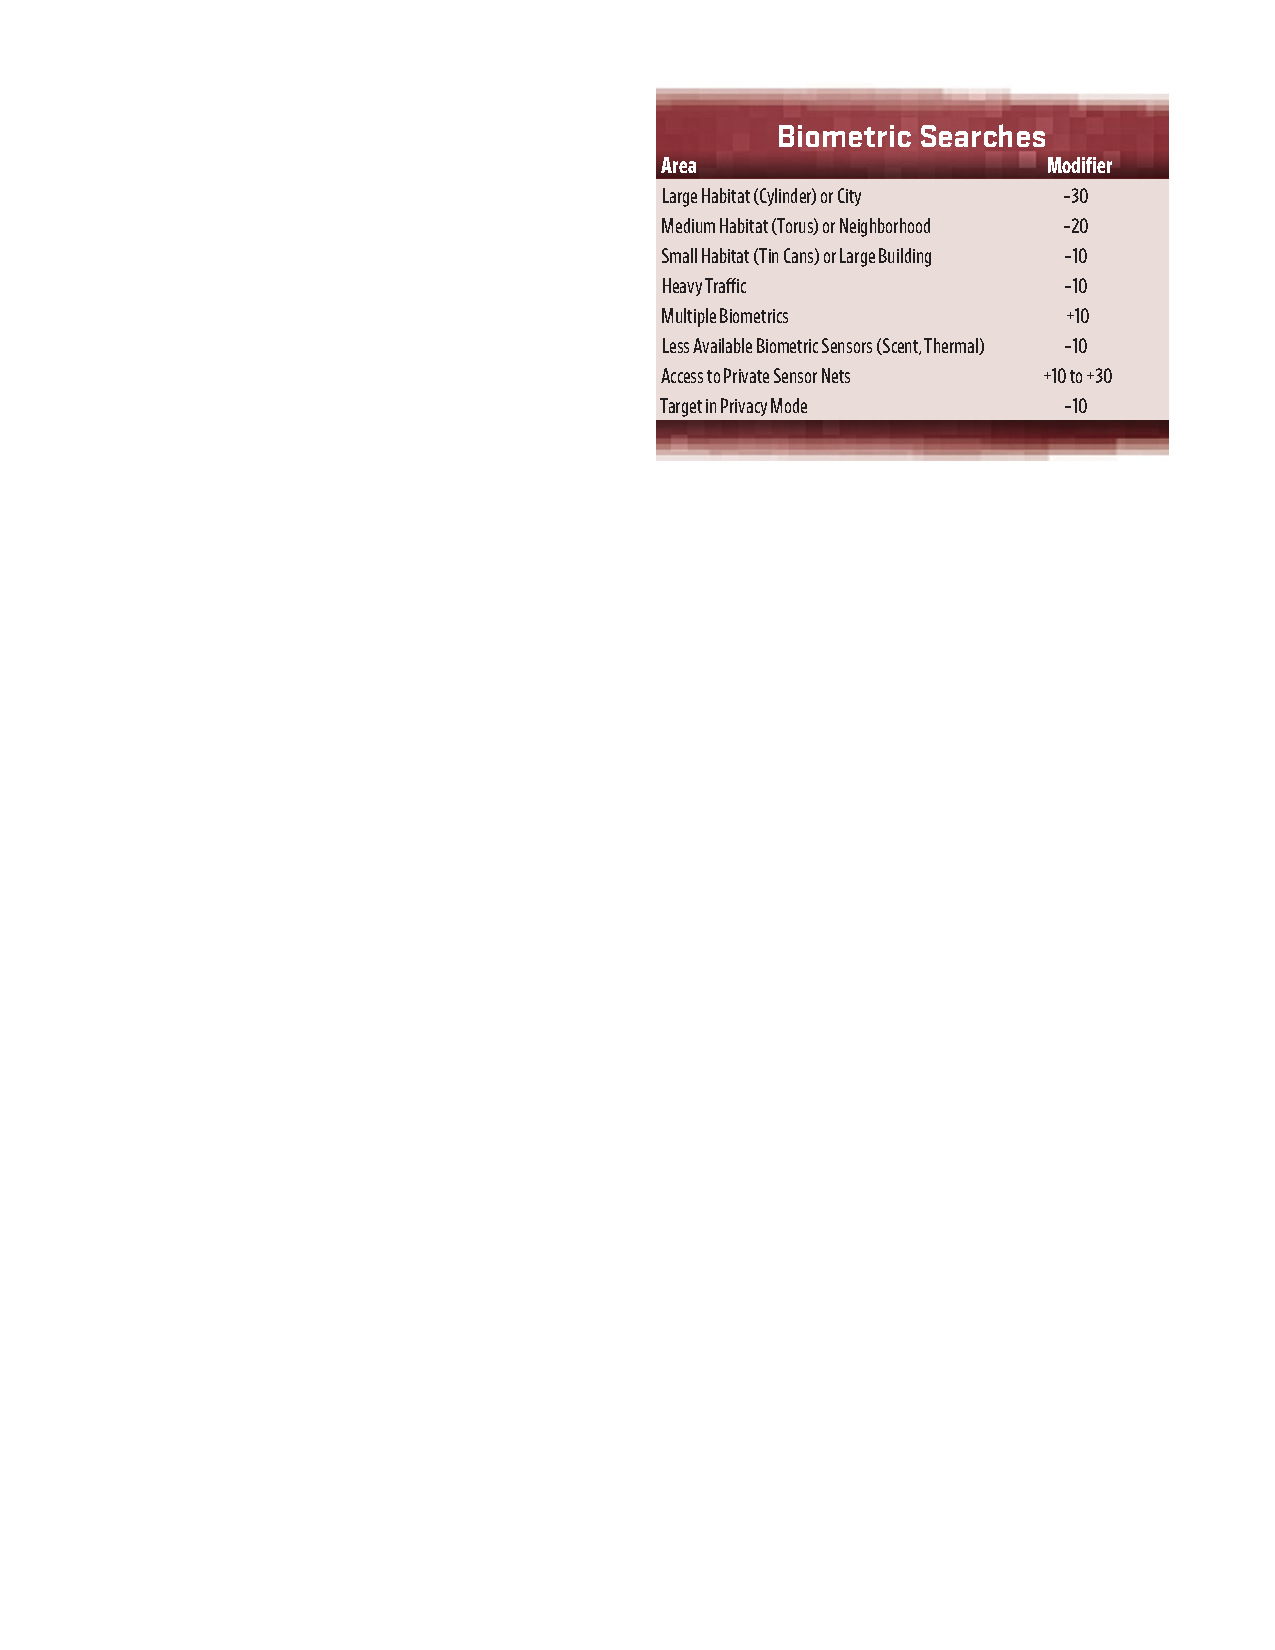
\includegraphics[scale=1.0]{gfx/mesh-search-biometric}%
\end{figure}%

\subsection*{Mesh Tracking}

\begin{itemize}
   \itembox Public information easily accessible, private info might require \skill{Research} scraping at \modifier{-30}, favors, or special database access.
   \itembox Live activity tracking can generally be difficult (\skill{Research} at \modifier{-30}) or impossible even if mesh ID is known. Better approach is to sniff traffic or hack their PAN. Tracking activity on particular system can be done with elevated accounts.
   \itembox Countermeasures are burner mesh IDs, disposable Ectos, VPNs, anonymizing proxies and spoofing mesh IDs.
\end{itemize}


\subsection*{Intrusion}

\begin{eptable}{ l | X }
   \epheader{2}{Ways of Hacking}
   Circumvent Authentication & Gain or forge access tokens.\\
   Spoofing & Intercept traffic and impersonate user.\\
   Intrusion & Find exploits to gain access.\\
\end{eptable}

\bigskip

\begin{itemize}
   \itembox Intrusion first requires a direct connection, either wirelessly (need to know target mesh ID), via an access port, or via tapping into a cable (\skill{Hardware: Electronics}).
   \itembox Brute force hacking is complex action, Hacking test, at \modifier{-30}. If successful get user access level (each superior upgrades access level). Attacker is in \textit{spotted} status, system goes into alert. On critical success \textit{covert} status.
   \itembox Subtle hacking has \SI{1}{h} task action, success grants user access level.
\end{itemize}

\begin{figure}[htbp!]%
   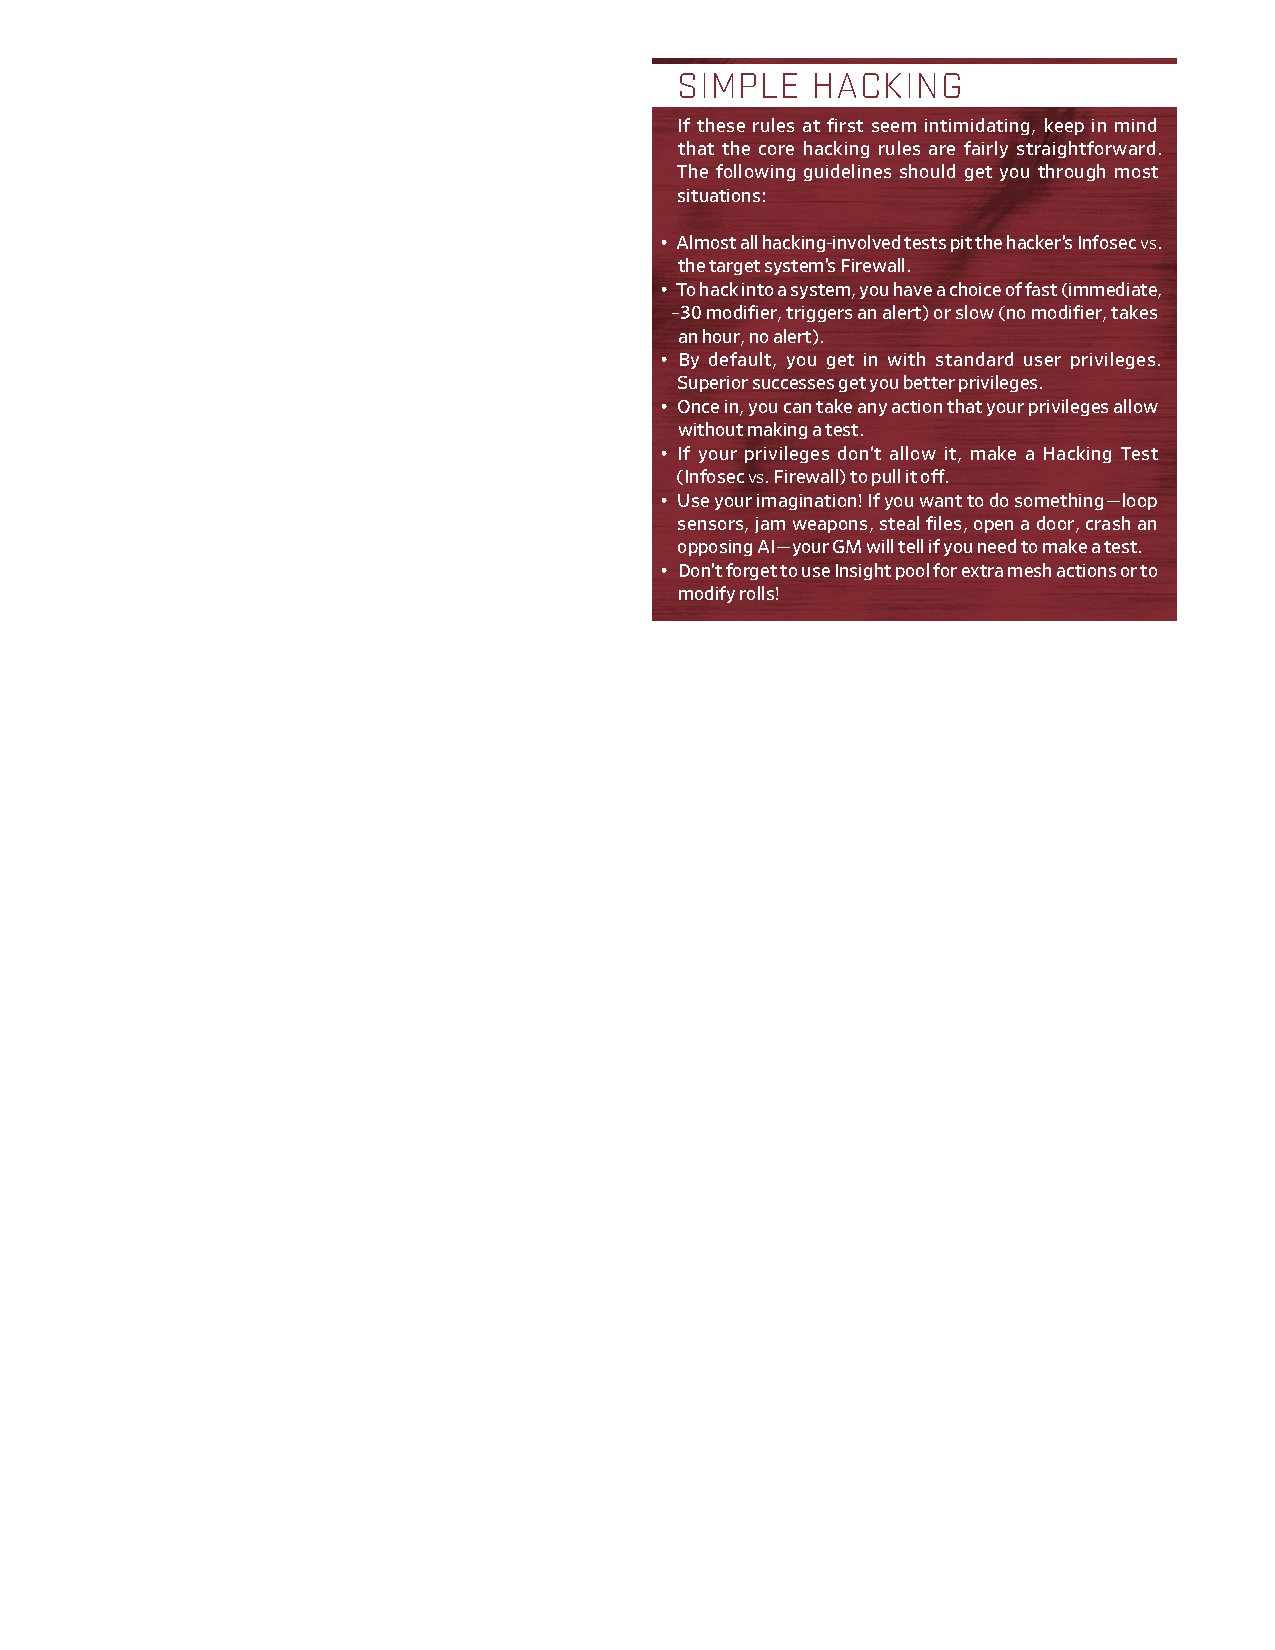
\includegraphics[scale=1.0]{gfx/mesh-hacking}%
\end{figure}%


\begin{figure}[htbp!]%
   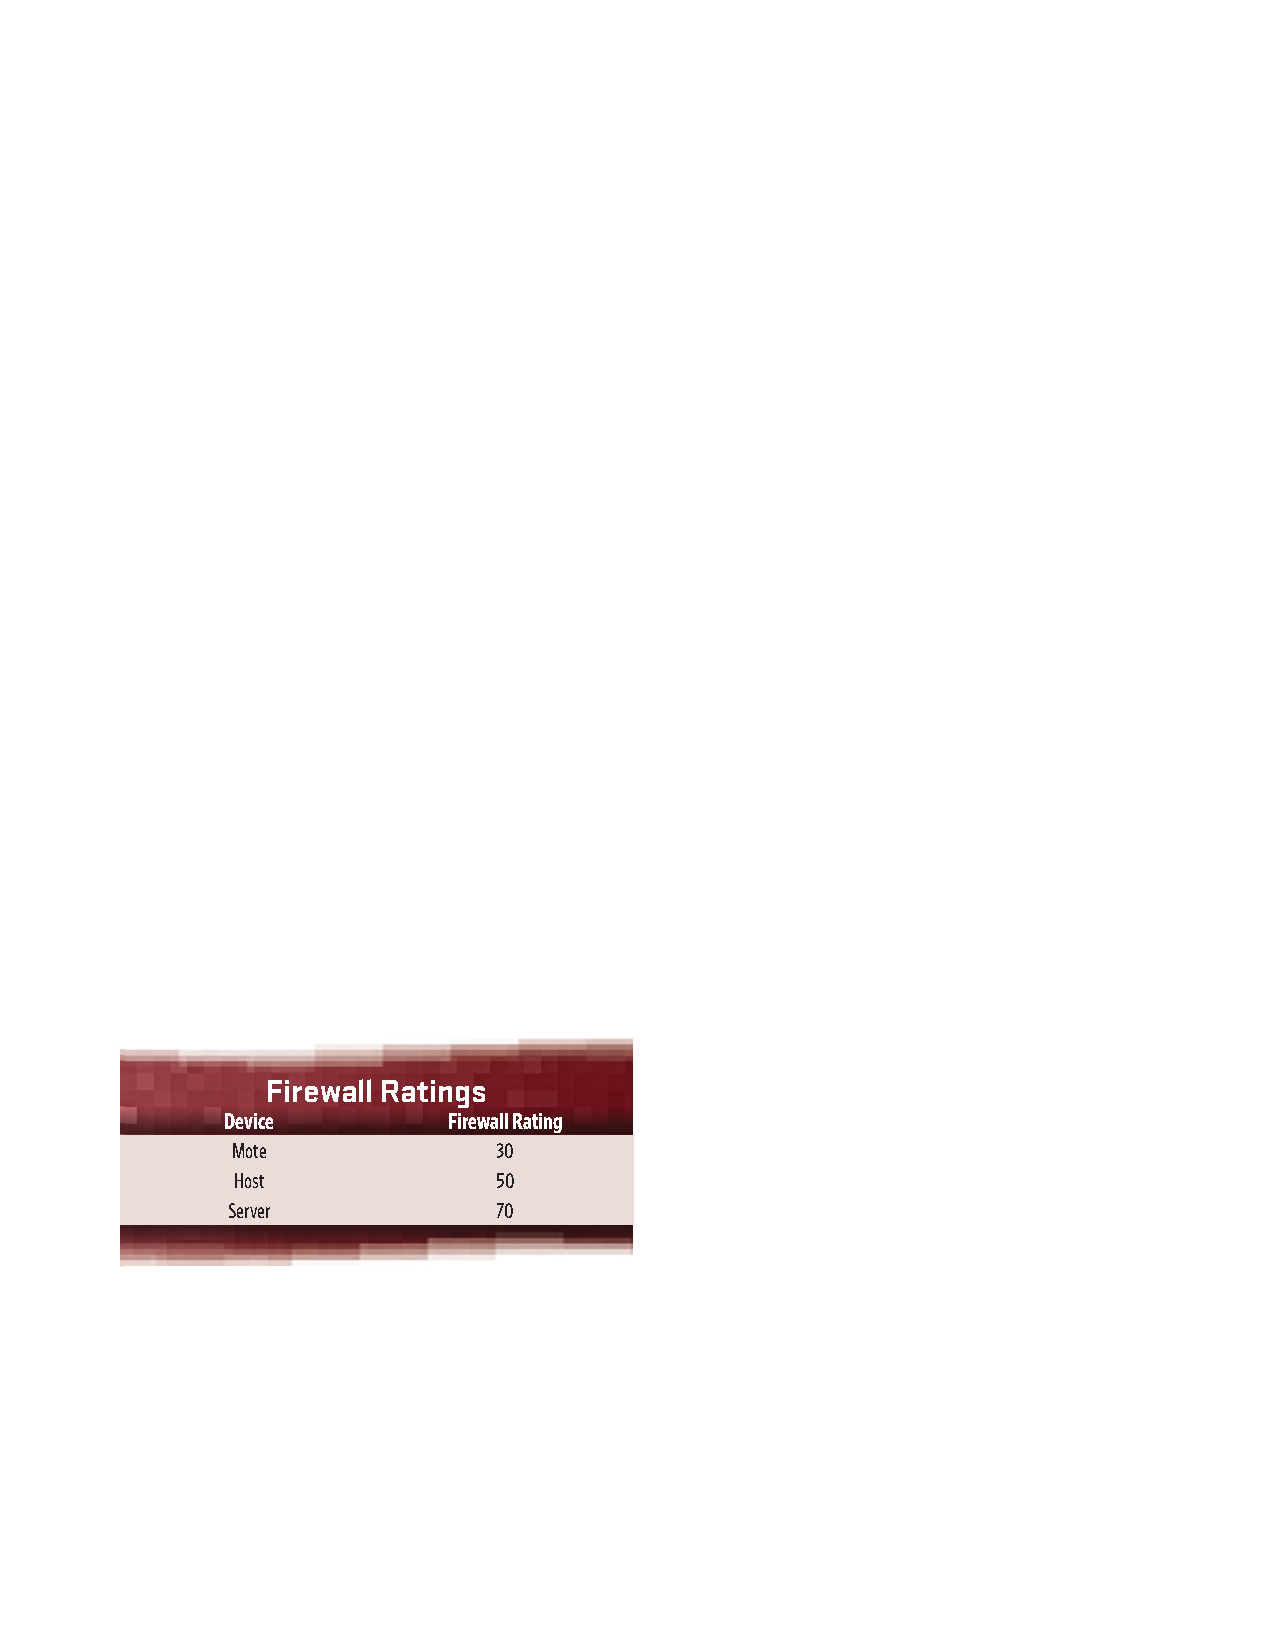
\includegraphics[scale=1.0]{gfx/mesh-firewall}%
\end{figure}%


\begin{eptable}{ l | X }
   \epheader{2}{Intruder Status}
    Hidden & System completely unaware. Get +10 to subvert system.\\
    Covert & System aware of presence, but does not consider threat.\\
    Spotted & System considers threat, launches countermeasures.\\
\end{eptable}

\bigskip

\begin{itemize}
   \itembox Can spend complex action \skill{Hacking} to try to upgrade status. Does not erase logs, but makes harder to pinpoint attacker.
   \itembox Any \skill{Infosec} while within system risks exposure. Superior failure triggers passive alert, critical failure spotted status.
   \itembox To pinpoint intruder on passive alert, system may do opposed \skill{Infosec} against intruder. If successful, system goes active alert.
\end{itemize}


\begin{eptable}{ l | X }
   \epheader{2}{Security Alerts}
    Passive Alert & Notifies admin, might launch passive CM, usually \SI{10}{m} cooldown.\\
    Active Alert & Launches active CM, attacker suffer \modifier{-10}.\\
\end{eptable}

\bigskip

\begin{eptable}{ l | X }
   \epheader{2}{Passive Countermeasures}
    Backup & Back up all critical information to prevent deletion.\\
    Egress Filtering & Block outgoing transfers (contest w. \skill{Hacking}).\\
    Locate Intruder & Try to zero in on intruder in system.\\
    Reduce Privileges & Reduce access rights of standard users.\\
\end{eptable}

\bigskip

\begin{eptable}{ l | X }
   \epheader{2}{Active Countermeasures}
    Counter Intrusion & Try to back-hack intruder if identified.\\
    Crash and Lockout & Crash intruder shell and prevent further access.\\
    Reboot or Shutdown & Takes \dice{1d6} actions or minutes.\\
    Terminate Connections & System can't be accessed anymore.\\
    Trace & Try to identify attacker's physical location.\\
\end{eptable}


\begin{figure}[htb!]%
   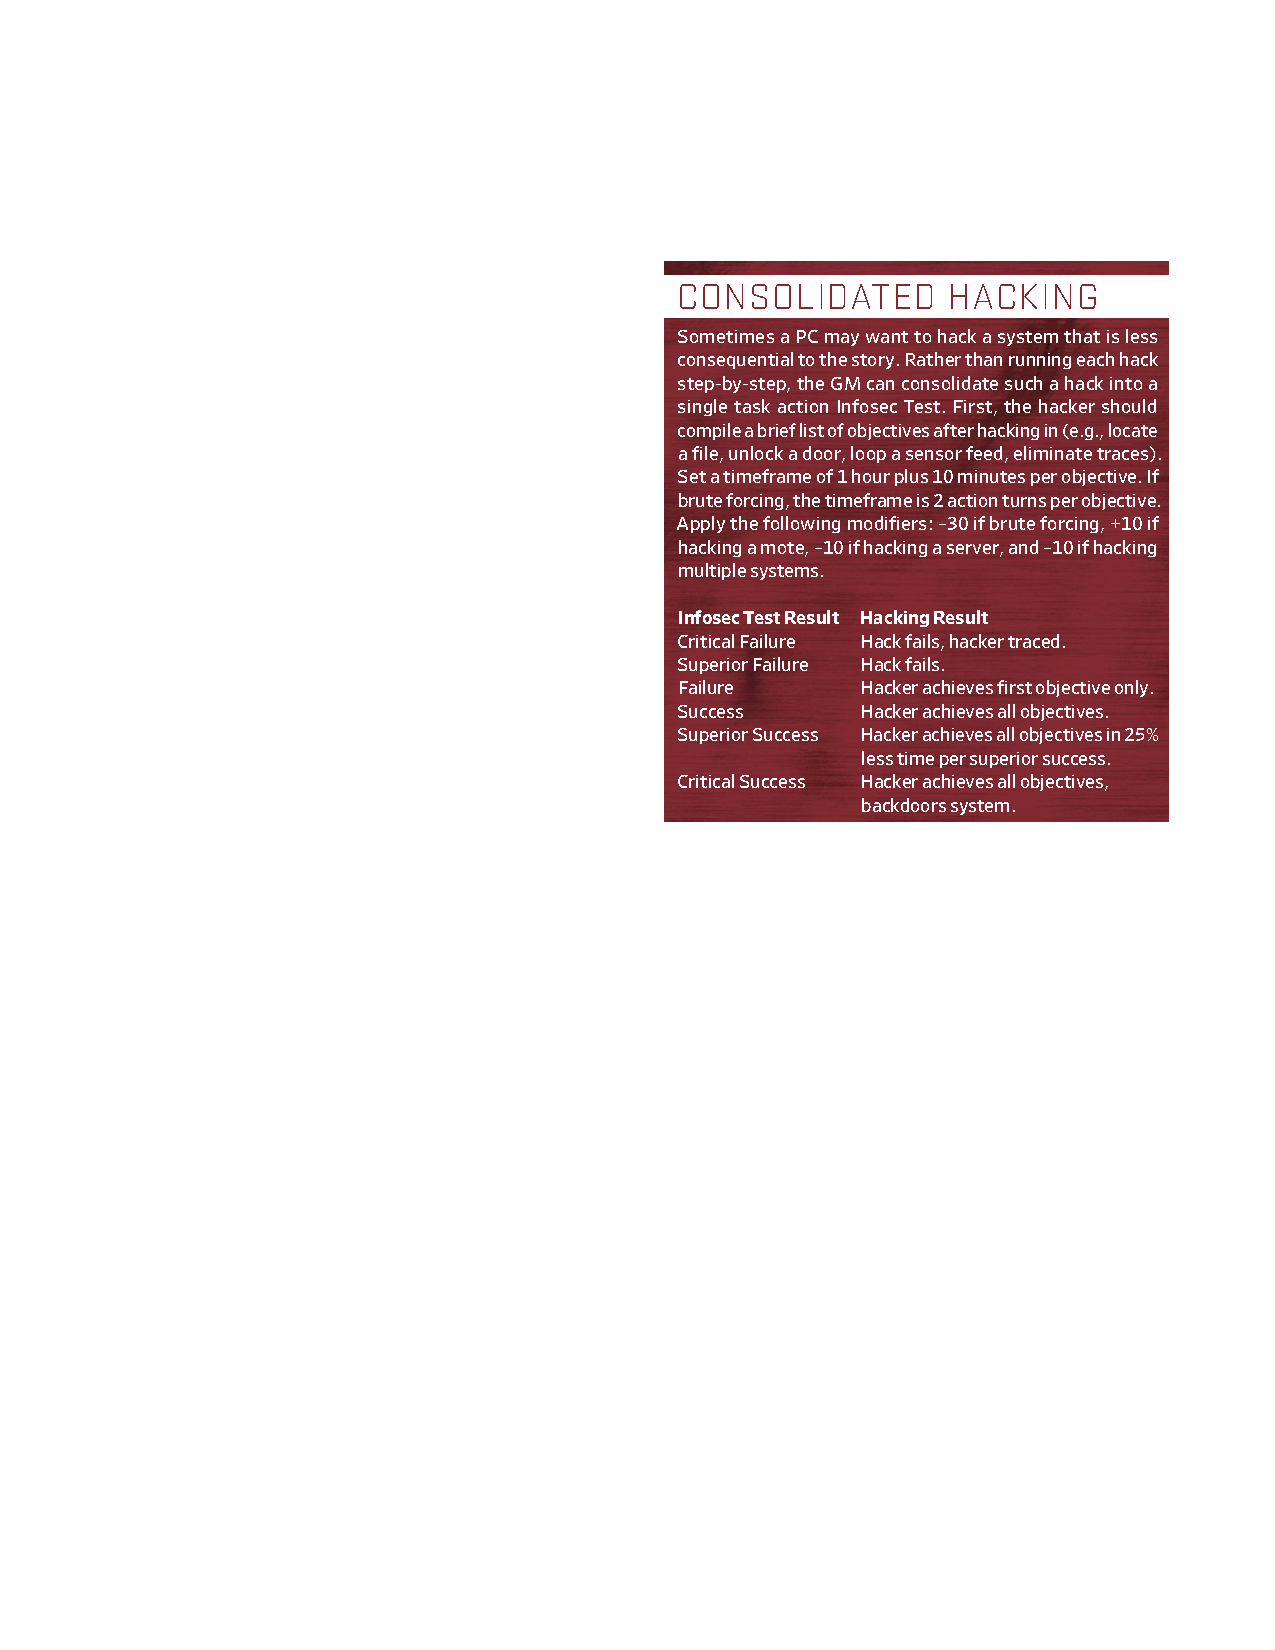
\includegraphics[scale=1.0]{gfx/mesh-consolidated-hacking}%
\end{figure}%

\bigskip

\subsection*{Subversion}

\begin{eptable}{ l | X }
   \epheader{2}{Subversion}
   Break Encryption & View all non-hidden users.\\
   Control Ware & Modify user hardware.\\
   Disable Safety Mechanics & Disable system preventing accidental harm.\\
   Edit AR Feed & Block or override user's sensory data.\\
   Eliminate Traces & Clean up evidence of break in.\\
   Force Re-Authentication & Can be used to sniff user's credentials.\\
   Hide File or Process & Makes it harder to find later.\\
   Impair Senses & Can induce \modifier{-10} modifiers to perception.\\
   Inject AR Illusion & Crafted in advance for best results.\\
   Install Backdoor & Bypass authentication later.\\
   Install Blocker & Block apps and countermeasures.\\
   Jam Signals & Interfere with local communications.\\
   Loop Sensor Feed & Undermine surveillance.\\
   Modify Tacnet & Change enemy's status information. \\
   Sniff Traffic & See above. \\
   Suppress Alarm & Turn off passive alarm or reduce active to passive. \\
   Suppress Process & Prevent process from coming back on again. \\
   Tap AR & See other user's AR feed as if it were your own. \\
   Tap Senses & Tap into cyberbrain or mesh insert senses. \\
\end{eptable}

\bigskip

Subversion is usually handled as \skill{Hacking} test.

\subsection*{Mesh Combat}

\begin{itemize}
   \itembox Works somewhat like regular combat. \textbf{Local attacks} require access and account on system and can attack entities on system. \textbf{Remote attacks} attack operating systems of remote devices, but cannot attack infomorphs, cyberbrains, or software running on them.
   \itembox Attack is complex \skill{Infosec}. If local attack and you do not have admin, you suffer \modifier{-30}. If system is shielding, opposed \skill{Infosec} roll. Remote attacks are opposed by \skill{Firewall} or defender \skill{Infosec}.
   \itembox Attacks are not obvious but rather glitches. Victim can't fight back unless \skill{Infosec} complex action to identify attacker.
   \itembox Mesh damage is \dice{2d10}, added \dice{1d6} per superior, double for critical.
   \itembox Wound mechanic similar to regular wounds, including cumulative \modifier{-10} modifier. Each wound causes cumulative \SI{10}{\%} chance for system glitch.
   \itembox Apps can't heal and need to restart. Infomorphs and others heal \dice{1d10} or 1 wound per minute.
\end{itemize}

\bigskip

\begin{eptable}{ l | X }
   \epheader{2}{Glitch Table}
    1 - 2 & Lost Connectivity. If cyberbrain, collapses or freezes.\\
    3 & Encoding Error. Might get spotted, leak real ID, compromise system.\\
    4 & Memory Loss. Might lose file, memory or skill until reboot.\\
    5 & Hung Process. App or synthmorph system might stop working.\\
    6 & Overload. Can't use pool for \dice{1d6}, or function every other round.\\
\end{eptable}


\begin{figure}[htb!]%
   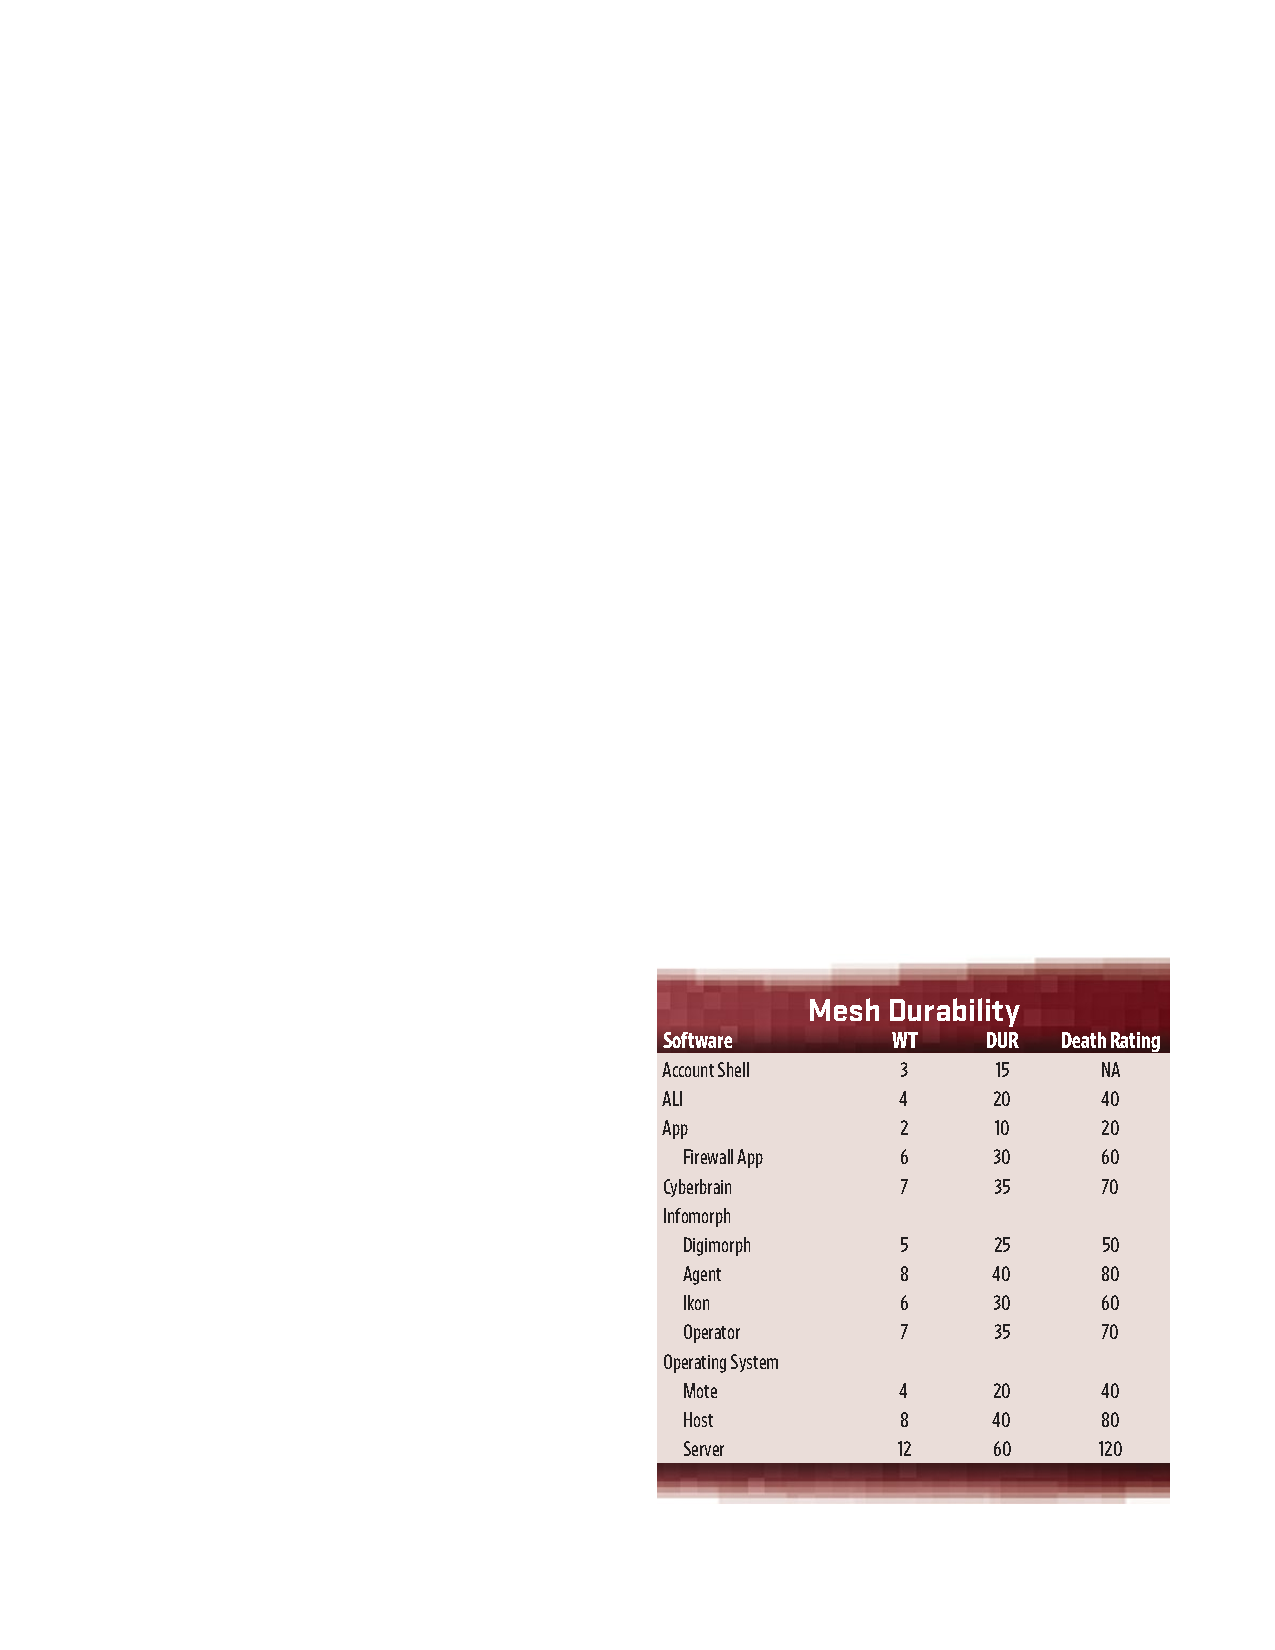
\includegraphics[scale=1.0]{gfx/mesh-combat}%
\end{figure}%